\chapter{Lecture 9}

%--- 信息 ----
\begin{center}
    讲师:王立威 \qquad
    课程时间:25.Apr.15th \qquad 
    笔记:25.June.9th
\end{center}

\bigskip

首先回答了上一节的最后一个例子,我已经放在了前面的讨论中. 

这个例子其实给了我们一个设计上的启发,$\Null(H)$中一共有$2^{7-3}=16$个元素,将这些元素作为码字可以保证其两两距离均大于等于$3$,因此足够纠正1比特的错误!由此定义Hamming码: 

\begin{definition}[Hamming $(n,m)$码]
    对于某个正整数$t$,我们记$1, 2, \dots, 2^t-1$的二进制列向量表达为$v_1, v_2, \dots, v_{2^t-1}$,得到矩阵 
    \[
H = \begin{bmatrix}
    v_1, & v_2, & \cdots & ,v_{2^t-1}
\end{bmatrix}_{t \times 2^t-1}
    \]

    该矩阵的零空间$\Null(H)$中的所有元素作为码字称作Hamming$(n,r)$码,其中$n=2^t-1, m=2^t-t-1$. 
\end{definition}

上一个例子中的给出的就是Hamming $(7,4)$码,是极其常用的. 并且它完美契合了之前得到的下界.  
\begin{definition}[完美码]
    对于一个码$C$,如果达到了球形邻域给出的下界,则称其为\textbf{完美码}(perfect code). 即要满足 
    \[
        2^n = 2^m \cdot \sum_{i=1}^t \binom{n}{i}
    \]
\end{definition}
\begin{theorem}
    Hamming码是完美码.
\end{theorem}
\begin{solution}
    请读者对Hamming $(7,4)$码自行验证. 
\end{solution}

现在来考虑如何解码,事实上这需要将不在码字中的元素映射到最近邻的码字,如下图所示:
\begin{figure}[H]
    \centering
    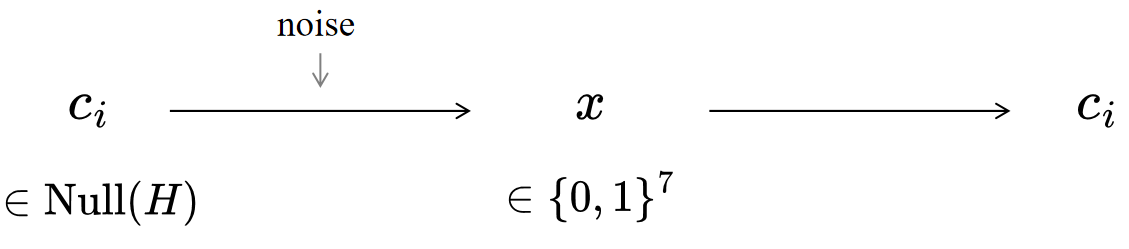
\includegraphics[width=.8\textwidth]{images/c9_1.png}
    \caption{解码图示}
\end{figure}

如果$d_H(x, c_i) \le 1$bit,那么只有两种情况,如果$x=c_i$,那么$Hx=0$;如果$x = c_i + \bm{e}_j$其中$\bm{e}_j$是仅在第$j$位上是1,其余全是0的向量,那么$Hx = Hc_i + H\bm{e}_j = v_j$. 对于后者的情况,我们可以轻易从$v_j$中推断出$j$,只需要取$c_i = x - v_j$即可. 这也说明了我们按二进制排序$H$的列向量的合理性,于是我们称这个$H$为\textbf{校验矩阵}(check matrix). 

下面考虑编码的方法,一个十分理想的编码是将消息$m_i$映射到码字$c_i$,其中保证$m_i$是$c_i$的部分前缀(换言之$c_i$的前$m$位就是$m_i$)我们现在取$\Null(H)$的一组基$\{g_i\}_i$,这组基的大小应该是$m$,记 
\[
G = \begin{bmatrix}
    g_1, & g_2, & \cdots ,g_{m}
\end{bmatrix}_{n \times m}
\]
我们规定编码的映射$f$如下:
\[
f(a) = \sum_{i=1}^4 a_i g_i = Ga \in \Null(H)
\]
我们称这样的$G$为\textbf{生成矩阵}(generator matrix). 

\begin{theorem}
    生成矩阵$G$和校验矩阵$H$满足$HG=O$
\end{theorem}
\begin{proof}
    这个定理十分显然,因为$Hg_i= 0$ 对于任意$i$.
\end{proof}

但至此我们还没有保证$c_i$的前$m$位就是$m_i$,但思考一下,我们只需要$G$具有如下形式即可:
\[
G = \left[\begin{array}{c}
I_{m \times m} \\ \hline 
\tilde{G}_{(n-m)\times m}
\end{array}\right] \quad \Ra \quad 
Ga = \left[\begin{array}{c}
a \\ \hline 
\tilde{G}a
\end{array}\right]
\]
当然只要$G$是满秩的,我们就可以将其上部的方阵调整为单位矩阵. 

下面接着介绍另一种码,线性码. 它是一种更广泛的定义,记作$[n,k,d]$码,$n$是长度,$k$是维度,$d$是Hamming距离. 具体而言:
\begin{definition}[线性码]
    一个\textbf{线性码}(linear code)是$\{0,1\}^n$的一个$k$维子空间,满足这个空间中任意两个不同元素之间的Hamming距离都大于等于$d$.  这样的码记作$[n,k,d]$码. 
\end{definition}
\begin{example}
    之前提到的Hamming $(7,4)$码,其实是一个$[7,4,3]$码.
\end{example} 

在线性码中,编码的步骤也是这样的,有一个生成矩阵$G_{n\times k}$,其列向量就是子空间的一组基. 

回到原来的Hamming码,我们有一组标准的方式构造$H$和$G$,这样的得到的码称作系统码或标准码:
\begin{definition}[系统码]
    一组\textbf{系统码}(systematic code)是由如下形式的$G,H$生成的:
    \[
G = \left[\begin{array}{c}
I_{m \times m} \\ \hline 
P_{(n-m)\times m}
\end{array}\right] ,\quad 
H = \left[\begin{array}{c|c}
P_{(n-m)\times m} & I_{(n-m)\times (n-m)}
\end{array}\right]
    \]
\end{definition}

当然并不是所有码都构成一个线性空间,也有大量的\textbf{非线性码},一般用$(n,M,d)$表记,其中$M$表示码字的个数(对应线性码中的$2^m$).  对于这样的码,方法生成新的码:
\begin{definition}[缩短]
    对于一组$(n,M,d)$码$C$,将其拆分为两个集合
    \[
    C_0 := \{c : c_n = 0\}, \quad C_1 := \{c : c_n = 1\}
    \]

    则其中必然有一个集合的元素个数大于等于$M/2$,取该集合中每个元素的前$n-1$位得到新的码$\tilde{C}$,是$(n-1,\tilde{M}, \tilde{d})$的. 一定有$\tilde{M} \ge M/2, \tilde{d}\ge d$. 这种方法称作\textbf{缩短}(shorten). 
\end{definition}

现在考虑与缩短相反的操作,对于一个$(n,M,d)$码$C$,满足$d$是奇数. 我们现在对于$C$中的每一个码字$c_i$,在后面添加一个比特$b$得到$\tilde{c}_i$,使得$\norm{\tilde{c}_i}_1$是偶数,这样一来码字之间的Hamming距离也必然是偶数,且不小于$d$,故不小于$d+1$. 因此如此得到的码$\tilde{C}$是$(n+1,M,\tilde{d})$的,满足$\tilde{d} \ge d+1$. 

\begin{example}
    试将Hamming $[7,4,3]$码改造为$[8,4,4]$码.
\end{example} 

最后,看一个例子(这里老师有一些混用$G$和$G^\top$的表记,大部分教材上使用的是将$g_i$作为行向量的版本,不过我相信只要提前声明这就是等价的)

\begin{example}
    考察这样的线性码生成矩阵,它和Hamming $[7,4,3]$码等价:
\[
G = \begin{bmatrix}
    1 & 1 & 0 & 1 & 0 & 0 & 0 \\
    0 & 1 & 1 & 0 & 1 & 0 & 0 \\
    0 & 0 & 1 & 1 & 0 & 1 & 0 \\
    0 & 0 & 0 & 1 & 1 & 0 & 1
\end{bmatrix}
\]
\end{example}


这样满足每一行都是上一行的位移的码,称作\textbf{循环码}(cyclic code). 有关于循环码的更多内容,若有兴趣请自行查阅.  